\documentclass{article}
 
\usepackage[spanish]{babel}
\usepackage{listings}
\usepackage{epsfig} 
\usepackage{float}
 \usepackage{hyperref}
 \usepackage{color}
\usepackage{graphicx} % figuras
\usepackage{subfigure} % subfiguras

%\usepackage{multicol}
%\usepackage{url}
%\renewcommand{\UrlFont}{\small}
\setlength{\parskip}{0.25 cm}
\setlength{\parindent}{0pt}


\title{Diseño de los grafos}
\author{1484166}
%\institute{PISIS UANL}
%\email{hhector.garcialpz@uanl.edu.mx}
\date{}


\begin{document}
\maketitle

\section*{Introducción}
Un grafo se puede dibujar de muchas maneras ya que por lo que representan aveces es conveniente verlo de cierto modo. En este documento se muestra algunas opciones presentes en la librería de \texttt{Networkx}

\definecolor{mygreen}{rgb}{0,0.6,0}
\definecolor{mygray}{rgb}{0.5,0.5,0.5}
\definecolor{mymauve}{rgb}{0.58,0,0.82}
\lstset{ 
  backgroundcolor=\color{white},   % choose the background color; you must add \usepackage{color} or \usepackage{xcolor}; should come as last argument
  basicstyle=\footnotesize,        % the size of the fonts that are used for the code
  breakatwhitespace=false,         % sets if automatic breaks should only happen at whitespace
  breaklines=true,                 % sets automatic line breaking
  captionpos=b,                    % sets the caption-position to bottom
  commentstyle=\color{mygreen},    % comment style
  deletekeywords={...},            % if you want to delete keywords from the given language
  escapeinside={\%*}{*)},          % if you want to add LaTeX within your code
  extendedchars=true,              % lets you use non-ASCII characters; for 8-bits encodings only, does not work with UTF-8
  firstnumber=1,                % start line enumeration with line 1000
  frame=single,	                   % adds a frame around the code
  keepspaces=true,                 % keeps spaces in text, useful for keeping indentation of code (possibly needs columns=flexible)
  keywordstyle=\color{blue},       % keyword style
  language=Octave,                 % the language of the code
  morekeywords={*,...},            % if you want to add more keywords to the set
  numbers=left,                    % where to put the line-numbers; possible values are (none, left, right)
  numbersep=5pt,                   % how far the line-numbers are from the code
  numberstyle=\tiny\color{mygray}, % the style that is used for the line-numbers
  rulecolor=\color{black},         % if not set, the frame-color may be changed on line-breaks within not-black text (e.g. comments (green here))
  showspaces=false,                % show spaces everywhere adding particular underscores; it overrides 'showstringspaces'
  showstringspaces=false,          % underline spaces within strings only
  showtabs=false,                  % show tabs within strings adding particular underscores
  stepnumber=1,                    % the step between two line-numbers. If it's 1, each line will be numbered
  stringstyle=\color{mymauve},     % string literal style
  tabsize=2,	                   % sets default tabsize to 2 spaces
  title=\lstname                   % show the filename of files included with \lstinputlisting; also try caption instead of title
}


%UNO...............
\section{Diseño bipartito}
Un grafo bipartito es aquel donde sus nodos se pueden repartir en dos conjuntos disjuntos.

\begin{figure}[h]
\centering
\includegraphics [width=100mm] {SSeptimo.eps}
\caption{Grafo bipartito}
\label{1}
\end{figure}

\begin{figure}[h]
\centering
\subfigure[Grafo bipartito]{\includegraphics[width=60mm]{CCuarto.eps}}
\subfigure[Grafo dirigido acíclico]{\includegraphics[width=60mm]{Cuarto.eps}}
\caption{Comparativa entre grafo con acomodo bipartito \texttt{vs} grafo con acomodo por default} \label{uno}
\end{figure}

\newpage{}
El código que da paso a la figura \ref{1} es el siguiente.
\lstinputlisting[language=Python, firstline=118, lastline=132]{Grafos_layout.py}


%DOS..........
\section{Diseño circular}
Como lo dice su nombre, un grafo de este tipo es el que tiene una distribución circular. Para hacer estos grafos se usa la función \texttt{circular\_layout()}

\begin{figure}[H]
\centering
\includegraphics [width=100mm] {NNoveno.eps}
\caption{Grafo circular}
\label{2}
\end{figure}

\begin{figure}[h]
\centering
\subfigure[Grafo circular]{\includegraphics[width=60mm]{SSegundo.eps}}
\subfigure[Grafo no dirigido ciclico]{\includegraphics[width=60mm]{Segundo.eps}}
\caption{Comparativa entre grafo con acomodo circular \texttt{vs} grafo acomodo por default} \label{dos}
\end{figure}

Para graficar la red de la figura \ref{dos}, grafo con red circular se utilizó el siguiente código.
\lstinputlisting[language=Python, firstline=35, lastline=41]{Grafos_layout.py}

%TRES...........
\section{Diseño spectral}
En este acomodo del grafo se utiliza los vectores propios de una matriz como coordenadas cartesianas de los nodos de la gráfica. Para acceder a este diseño de grafos basta con ingresar la función \texttt{spectral\_layout()}.

\begin{figure}[h]
\centering
\includegraphics [width=100mm] {PPrimero.eps}
\caption{Grafo spectral}
\label{3}
\end{figure}

\begin{figure}[h]
\centering
\subfigure[Grafo spectral]{\includegraphics[width=60mm]{DDoceavo.eps}}
\subfigure[Multigrafo dirigido reflexivo]{\includegraphics[width=60mm]{Doceavo.eps}}
\caption{Comparativa entre grafo con acomodo espectral \texttt{vs} grafo con acomodo por default} \label{tres}
\end{figure}

\newpage
El código con el que se hizo el grafo de la figura \ref{tres} con acomodo espectral es.
\lstinputlisting[language=Python, firstline=199, lastline=223]{Grafos_layout.py}


%CUATRO..............
\section{Diseño spring}
Esta función hace una analogía de las fuerzas de física, el objetivo de este algoritmo es encontrar un acomodo de los nodos donde se minimice la suma de las fuerzas. Para obtener este tipo de grafo se utiliza la función \texttt{spring\_layout()}. Algunos ejemplos de muestran a continuación.

\begin{figure}[H]
\centering
\includegraphics [width=100mm] {DDecimo.eps}
\caption{Grafo spring}
\label{4}
\end{figure}

\begin{figure}[h]
\centering
\subfigure[Grafo spring]{\includegraphics[width=60mm]{OOctavo.eps}}
\subfigure[Multigrafo no dirigido ciclico]{\includegraphics[width=60mm]{Octavo.eps}}
\caption{Comparativa entre grafo con acomodo spring \texttt{vs} grafo con acomodo por default} \label{cuatro}
\end{figure}

\newpage
El siguiente código muestra como se hace el grafo de la figura \ref{cuatro}.
\lstinputlisting[language=Python, firstline=136, lastline=144]{Grafos_layout.py}

%CINCO..........
\section{Diseño Kamada Kawai}
Este tipo diseño se utiliza cuando se quiere reducir el número de cruces de los aristas, como se muestra en los siguientes gráficos. Para hacer uso de este diseño se usa la función \texttt{kamada\_kawai\_layout()}.

\begin{figure}[H]
\centering
\includegraphics [width=100mm] {OOnceavo.eps}
\caption{Grafo con diseño Kamada Kawai}
\label{5}
\end{figure}

\begin{figure}[h]
\centering
\subfigure[Grafo diseño Kamada Kawai]{\includegraphics[width=60mm]{QQuinto.eps}}
\subfigure[Grafo dirigido cíclico]{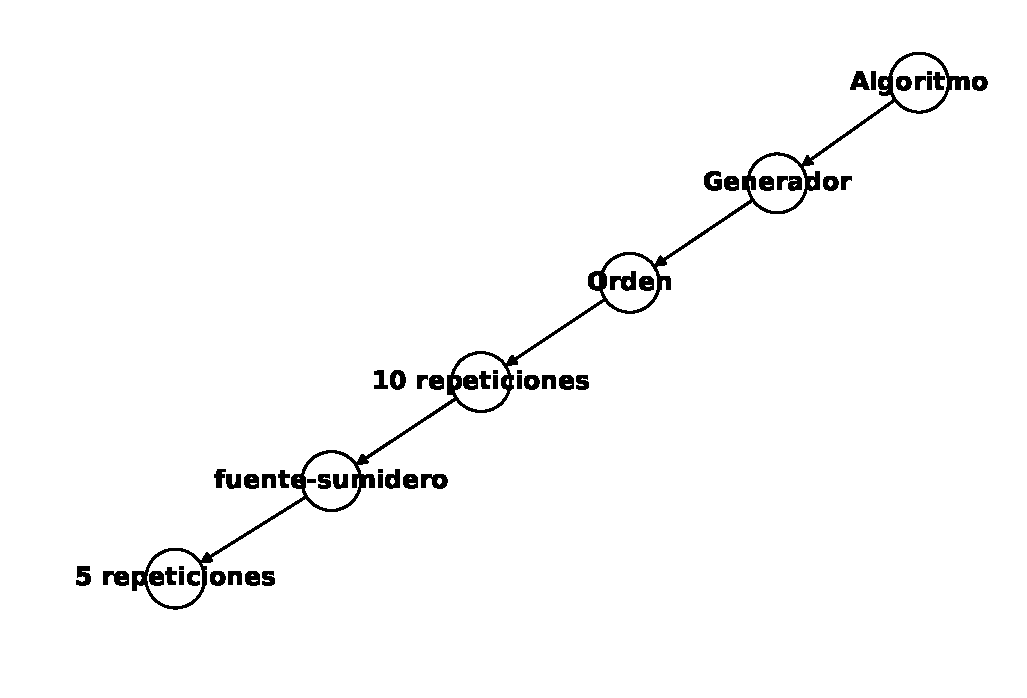
\includegraphics[width=60mm]{Quinto.eps}}
\caption{Comparativa entre grafo con acomodo Kamada Kawai \texttt{vs} grafo acomodo por default} \label{cinco}
\end{figure}

\newpage
El código con el que se hizo la red de la figura \ref{cinco} con el acomodo Kamada Kawai es.
\lstinputlisting[language=Python, firstline=86, lastline=94]{Grafos_layout.py}


%SEIS............
\section{Diseño shell}
Este algoritmo se basa en acomodar los nodos en circulos concéntricos.

\begin{figure}[H]
\centering
\includegraphics [width=100mm] {TTercero.eps}
\caption{Grafo dirigido reflexivo}
\label{6}
\end{figure}

\begin{figure}[h]
\centering
\subfigure[Grafo diseño shell]{\includegraphics[width=60mm]{SSexto.eps}}
\subfigure[Grafo dirigido cíclico]{\includegraphics[width=60mm]{Sexto.eps}}
\caption{Comparativa entre grafo con acomodo shell \texttt{vs} grafo acomodo por default} \label{seis}
\end{figure}

\newpage
Para hacer la red de la figura \ref{6} con el acomodo shell es.
\lstinputlisting[language=Python, firstline=45, lastline=67]{Grafos_layout.py}

\bibliographystyle{IEEEtran}
\bibliography{Bibliog}
\nocite{*}
\end{document}















